\section{Background} \label{background}

Multiple subjects lay at the base of the design described in section \ref{design}.

    \subsection{Electronic health record systems}

    Health information systems are becoming an important part of health care. They not only support patient care, but also administrative and financial tools. But at the heart of these systems lies the electronic health record. An electronic health record (EHR) is a repository of electronically maintained information about an individual's health status and health care, stored such that it can serve multiple legitimate uses and users of the record \cite{biomedical_informatics}. An electronic health record system (EHRS) provides tools to manage and interact with these records. These tools include providing reminders, data analysis and decision support. It helps the clinician to organize, interpret and react to data.

    First, the advantages of EHRS over paper-based records is described to signify its importance. Secondly, the main components present in these systems is summarized. The functionality of an EHRS can be categorized into two types: a monolithic system tries to provide more general care, while other systems cater to more specific care. The latter however, lacks certain functionalities or data, which requires the combined use of multiple systems. The last section compares the two types and highlights the benefits and drawbacks of both.

        % signify importance
        \subsubsection{Moving away from paper} \label{2_ehrs_paper}

        For modern medicine, the traditional paper-based medical records are not suited in today's world filled with technology. The drawbacks of information on paper are obvious when compared to digitally stored information.\\

        \noindent\textbf{Functionality} Digital records allow systems to aggregate, process and generate statistics of the data it contains. For example, heart rate graphs with typical statistics can be generated and when the users hovers over a data point in the graph, the exact value is shown. Paper records containing tables or printed graphs that show the same data are limited in this regard.

        A paper-based medical dossier can only store medical images, such as x-rays, but compared to a digital image, a lot of detail is lost. As such, other multimedia and other file types are can not be stored. With an EHRS, these file types can be attached with ease, provided the system supports them. Paired with the tools of the system, a lot more functionality can be achieved.

        In terms of data input, an EHRS can detect and prevent false data input. The system can make sure all necessary data fields filled in and in the correct format. This results in more complete and accurate data gathering with less errors.\\

        \noindent\textbf{Information quality} A summarizing paper noted that the use of EHRS leads to more complete, accurate, comprehensive and reliable data compared to paper-based records \cite{ehrs_summary}. As mentioned in the previous paragraph, a digital system can impose rules on data fields to avoid missing or entering wrong data. In terms of comprehensibility, poor handwriting leads to wrong or loss of information, which is avoided on digital systems.\\

        \noindent\textbf{Accessibility} Paper records are difficult to access because most of the time only one copy exists. Transferring these records to other branches or institutions therefore is difficult: the record has to be found in the often large medical dossier, has to be copied and then manually sent. Also, misfiling, flooding or fires can lead to irrecoverable loss of the data. Digital records avoids the last issue, but there can still be difficulties regarding data transfer as most institutions have their own database structures.

        Because digital storage increases accessibility significantly, security measurements have to be taken. If not, data can be stolen, deleted or even altered. This also adds to the complexity of developing EHRS.\\

        % wip
        \noindent\textbf{Efficiency} An important task of an EHRS is to facilitate efficient care. An early study saw a 6\% increase in productivity when EHRS were deployed in health care institutions \cite{ehrs_efficiency}. However, other factors are at play. One of these factors is adoption rate. The transition from paper-based documenting to digital is accompanied with a learning curve, which can be steep. After the switch, the productivity will be lower and as the users become more accustomed it will increase.

        The process of moving data on paper to a digital format requires a lot of manual work. While some aspects can be automated, such as scanning and processing paper forms, verification is still required. All the data fields from the documents need to find a place in the EHR, which frequently not possible. Also, what do we do with unreadable data due to poor handwriting? What happens with duplicate forms with slightly different values? Because of these reasons, adopting an EHRS is a significant undertaking for an institution. As such, the benefits are not immediately apparent.

        \subsubsection{Components of an EHRS}

        As mentioned before, EHRS do not simply store patient records. They consist of many components which ultimately define how well they perform in health care. Literature gives us multiple definitions of which components are essential. However, we summarize them in the following five \cite{biomedical_informatics}:\\

        \noindent\textbf{Integrated view of patient data} An EHR must allow storage of a wide range of data types. This can be text, numbers, images, video and others. Some data can still be on paper due to lacking support of the EHRS, as mentioned in section \ref{2_ehrs_paper}. To display more complex data types, such as x-ray images, standards are used. A brief overview of such standards can be found in section \ref{2_standards}.\\

        \noindent\textbf{Clinician order entry} Order entry is the point at which the clinician has to make decisions or take action. An order entry system can assist the clinician by providing decision support. It also reduces errors and costs compared to paper order entry.\\

        \noindent\textbf{Clinical decision support} A decision support system embed into an EHRS can aid the clinician by suggesting actions to take, when certain situations occur. If for example a patient is due for a vaccination, the system can notify the clinician by presenting a constructed order which needs to be confirmed or denied. The system can do this for a bulk of patients, so manual checkups are not required, thus saving time.\\

        \noindent\textbf{Access to knowledge resources} When clinicians are writing notes or orders for a patient, clinical questions can arise. Instead of asking colleagues, the EHRS can pull literature to address the question. Due to the internet, a very large source of information is readily available.\\

        \noindent\textbf{Integrated communication and reporting support} Communication is an important part in health care. Often clinicians of multiple institutions provide care for a particular patient. The effectiveness of patient care therefore is directly affected by communication which is why EHRS should provide tools to assist the clinicians. Most institutions are bounded by their own EHRS, which requires them to ask the other institutions for necessary data. A solution to this problem are Health Information Exchanges, which allows institutions to reach data beyond their own EHRS.\\
        
        \noindent Throughout the years, many EHRS have been developed which may or may not integrate all of the above components. If an essential component is missing, an institution may use another system. Although this has its benefits and drawbacks.

        \subsubsection{Monolithic vs. multiple EHRS} \label{ehrs_comparison}

        Health care institutions can opt for a monolithic EHRS or combine multiple EHRS to achieve all required functionality. To both there advantages and drawbacks \cite{multiple_ehrs}. Elements influencing this choice include IT infrastructure, safety risks, volume of care and frequency with which patients move facilities. However, it's possible that a single EHRS does not satisfy the requirements of an institution. A reason for this is that certain branches require specially tailored software for their clinical practice, which a general EHRS lacks. 

        Functionality wise, a monolithic EHRS tends to appeal to more general types of care, whereas it lacks in very specific ones. Also, vendors that offer these all-in-one solutions have less experience with these specialties which reduces the chance it will be added to the system. Vendors of specific EHRS do have this expertise and can tailor the system to the needs of the customer. In this case, combining a system that supports general care with special care systems will seem like the best choice. However, other considerations have to be made.

        The advantages of a monolithic system is that the data it uses is centralized. This ensures that all data can be accessible anywhere in the system and that it can be easier maintained. When multiple systems are in place, data has to be exchanged and can lead to difficulties finding certain pieces of information. The exchange of data is difficult, as each system probably has its own data structures. A potential solution is to create a new EHRS, solely for the purpose data collection and transformation with which all systems interface with. This leads to another system, requiring development and maintenance time.
    \subsection{Telemonitoring} \label{2_telemonitoring}
    % between consultations
    % devices, parameters
    Monitoring patients at a distance with the use of information technology is called telemonitoring \cite{telemonitoring_definition}. The rise of mobile devices such as smartphones and smartwatches made telemonitoring considerably more feasible. It allows the clinician to follow up on certain parameters, without having to schedule an appointment for a manual checkup. This saves both time and money, improving health care significantly.
    
    Telemonitoring can be applied anywhere the measuring devices allow it. This can be at home, work or during physical activity, allowing continuous monitoring of various parameters which would otherwise not have been documented. As a result, clinicians can gain insight into what happens between two consultations, which can be detrimental when providing care.
    
        \subsubsection{Devices \& parameters}

        test

    % integrate in EHRS
    % devices
    % parameters
    % data trustworthy?

    

    \subsection{Dashboards}

    \subsection{Customization}
    % effect on user satisfaction

    \subsection{Standards} \label{2_standards}

    \subsection{Privacy}
    % not focus, brief description of issues
    Although privacy is not a main focus, it is important to describe the topic concerning health informatics.

    \subsection{MuiCSer} \label{2_muicser}
    % description of process
    This section describes the MuiCSer framework, made for user-centred software engineering processes in a multidisciplinary context \cite{muicser}, which will be used to create the prototype. This framework focuses on optimizing the user experience during the entire software engineering cycle to ensure that the end-user's needs are fulfilled. By combining user-centred design and software engineering principles the user experience of the final product can be improved substantially of the final product.

        \subsubsection{Process}
        
        \begin{figure}[!t]
            \centering
            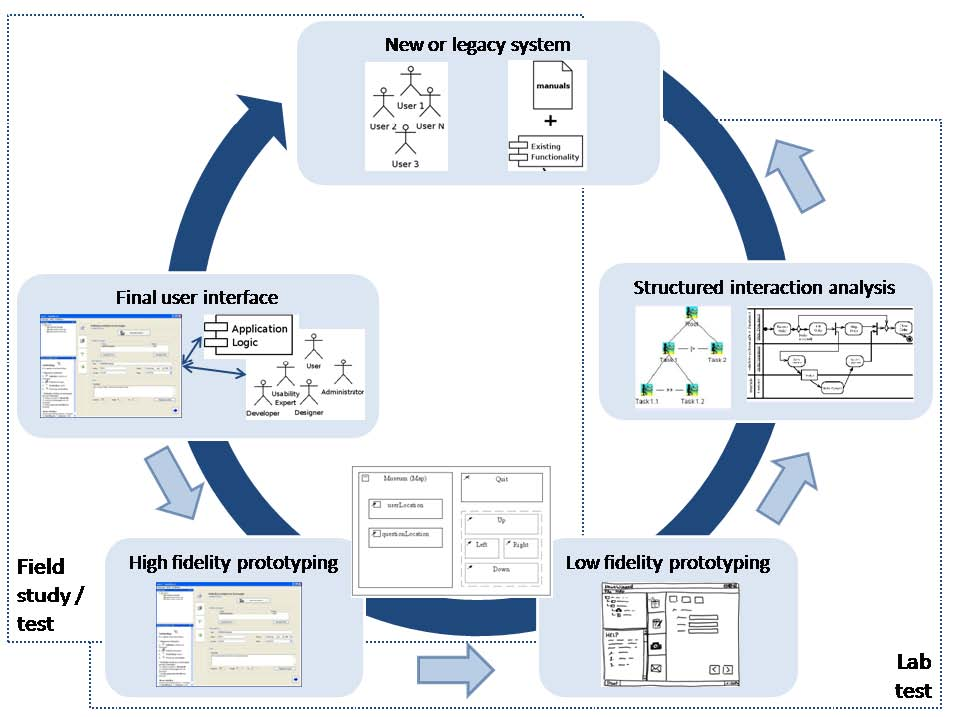
\includegraphics[width=0.8\textwidth]{chapters/2_background/muicser}
            \caption{MuiCSer process}\label{fig:muicser}
        \end{figure}

        The MuiCSer process is summarized in figure \ref{fig:muicser}. After each phase, the result is evaluated, verified and validated to ensure that the required functionality is present. The received feedback can in turn be used to reiterate over the previous phase. On the figure this is denoted with the light arrows, while the dark one represents the overall process direction.\\

        \noindent\textbf{New or legacy system} At the start of the process an existing system in need of improvement is either evaluated or a new one has to be designed. This requires an analysis of the tasks and needs of the user, as well as the objects and resources required to perform these tasks. Personas and scenarios are the resulting artifacts of this phase. First, personas describe the personalities of the potential end users including hobbies, skills and the environment they surround themselves in \cite{persona_scenario}. Its goal is to uncover behavior patterns which can be of use when designing a user interface. Second, a scenario is a story describing the use of a fictitious system from the persona's point of view \cite{persona_scenario}. It tries to sketch the usage of the system for which a design must be made.\\

        \noindent\textbf{Structured interaction analysis} During this phase, the results of the analysis are used to create task models. These models specify concrete tasks and goals which can be dissected into specific actions or steps the user has to take. These artifacts lay the foundation for designing a user interface which supports these tasks and goals.\\

        \noindent\textbf{Low fidelity prototyping} When the actions have been specified using the task models, low fidelity prototypes can be designed. Paper sketches and mockups are such examples and are ideal for visualizing the layout of the software its user interface. Without spending too much time and resources, presenting such prototypes can yield valuable feedback from the end-user or customer. However, there is no interaction present. Typically multiple versions of these prototypes will be created until the customer is satisfied after which high fidelity prototypes can be developed.\\

        \noindent\textbf{High fidelity prototyping} Creating high fidelity prototypes requires a lot more effort compared to low fidelity prototypes, as they offer functionality closely resembling the final product. However, the feedback given by the testers can be more elaborate. Not only design, but also functionality can be tested and criticized.\\

        \noindent\textbf{Final user interface} When the latest iteration of the high fidelity prototype satisfies all user requirements, the final user interface can be created. It would be beneficial to reuse the code from the prototype in order to save time and resources. As a final step, the task models are checked against the interface to check if all required functionality is present.\\


        

        


